\section{Materialization of Interactive Machine Learning Workloads} \label{sec-expert-expert}
Interactive machine learning workload requires fast response.
Typically users would analyze the data by first performing an exploratory analysis.
Then, based on these analyses, they apply the right set of transformations to the data to train one or multiple models on the transformed training data.
Using the experiment database, we can enhance the performance. 
By analyzing the experiment database we can extract the common transformations on data and materialize them.
When new users execute their workloads, we first analyze the workload to look for reuse opportunities and return the materialized data when possible.

We analyzed several scripts from the Titanic: Machine Learning from Disaster competition in Kaggle\footnote{https://www.kaggle.com/c/titanic}.
The Kaggle platform allows users to submit their solutions as scripts (called notebooks or kernels) to the Kaggle platform.
These notebooks are available publicly for other users to view and fork in their own workspace.
Figure \ref{fig-titanic-script-hierarchy} shows some of the popular notebooks and how other users wrote their notebooks based on the existing ones.
The numbers show how many times each script is forked.
The top most-voted notebooks for the Titanic competition have been forked a total of 44,434 times.
This demonstrates that many of the workloads share similar sets of data transformations and model training.
Materializing frequent transformations and models can greatly increase the efficiency and many repeated operations can be avoided.

\begin{figure}
\centering
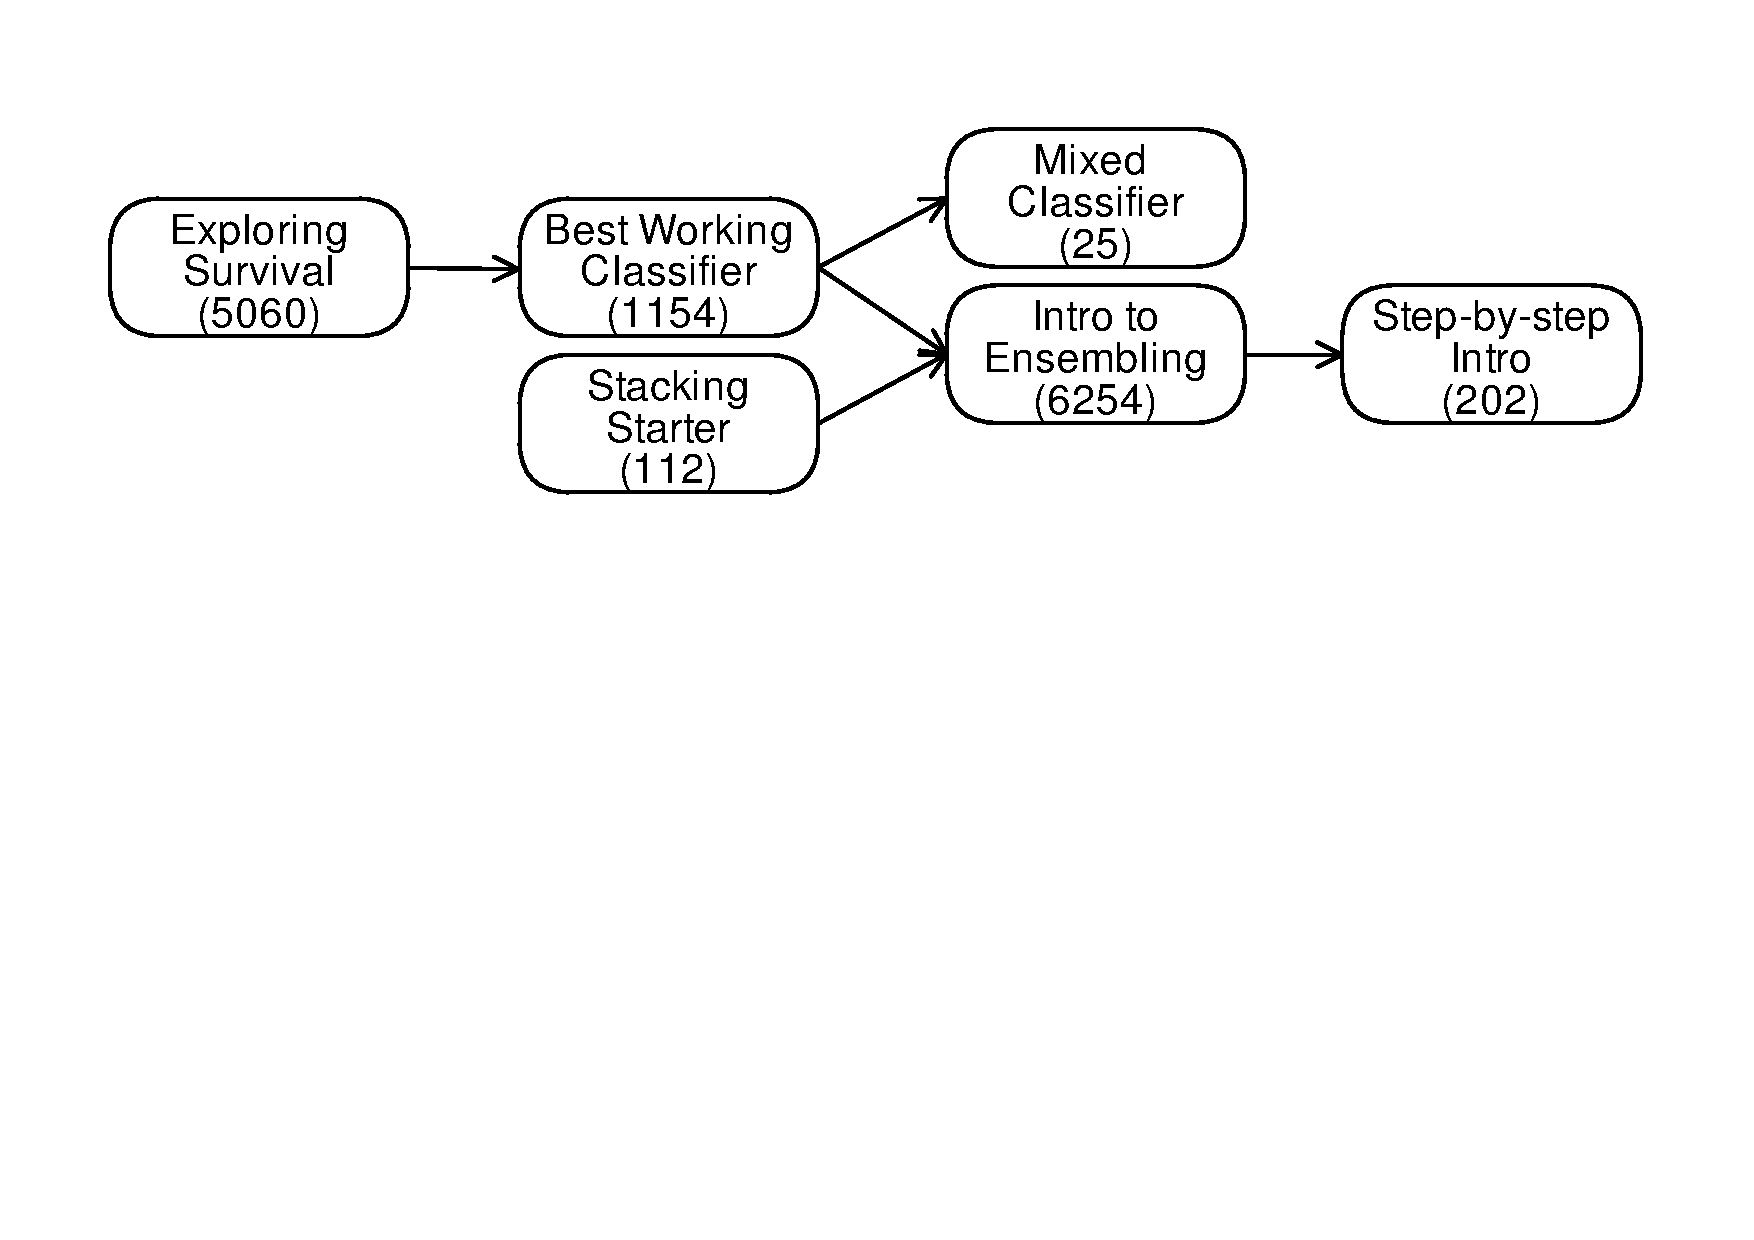
\includegraphics[width=\columnwidth]{../images/kaggle-titanic-scripts-graph}
\caption{The fork hierarchy of some of the popular notebooks in Kaggle's Titanic competition and how many times each notebook is forked}
\label{fig-titanic-script-hierarchy}
\end{figure}

In order to apply the materialization optimization, we first define the characteristics of the interactive machine learning workloads.
Then, we specify how to detect reuse opportunities from the experiment database.

\subsection{Interactive Machine Learning Workload Characteristics}
We assume the main units of work are dataframe like objects that contain one or many columns, where all the items in one column are of one data type.
We divide the operations in interactive ML workloads into 2 categories.

\textbf{1. Feature engineering:}
\begin{itemize}
\item feature selection operation that selects a set of features (columns) from the dataset
\item feature transformation that applies a function to a set of columns from the dataset and generates new columns
\end{itemize}


\textbf{2. Model building: }
\begin{itemize}
\item model training that applies a training algorithm to a dataset
\item aggregation operation that aggregates a set of columns based on the values in another column
\end{itemize}
Each model building operation results in objects (vertices) that can either be used in other feature engineering operations (applying PCA to data or categorization the data based on percentile values) or can be a complete machine learning model that can be used to make predictions on unseen data.
\todo[inline]{How can we capture these in the graph? maybe special edges that connect these nodes to a data node? }

\todo[inline]{In the rest of this section, I only mention materialization for the feature engineering operations. I have some ideas for the model building operations as well, but I will skip that for now. }

%%% Continue from here
\subsection{Graph Construction}
To construct the experiment graph, we first analyze each feature engineering or model building operation, then create the vertex and edge.
A transformation is defined as \textit{transform(d, i\_columns, func, o\_columns)}, where $d$ represents the dataset, $i\_columns$ represents the list of input columns, $func$ represents the function to be applied to those columns, and $o\_columns$ represents the output columns.
Datasets are represented as vertices and a transformation that maps a dataset to another are represented as edges.
Each vertex node contains a reference to the dataset and the list of the columns that dataset contains.
Each edge contains the transformation function ($tf$) and list of columns ($active\_columns$).
We define the model building operations with two methods.
Training a machine learning model is defined as \textit{train(d, alg)} which trains a model using the $alg$ on the given data $d$.
An aggregation operations is defined as \textit{aggr(d, i\_columns, func)}, which performs a groupby on the input columns ($i\_columns$) and aggregate the groups using the $func$ function.
Figure \ref{fig-experiment-graph} shows an example graph constructed from the code in Listing \ref{listing-experiment-graph}.
The script is based on the \textit{Titanic Best Working Classifier} from the Kaggle competition\footnote{https://www.kaggle.com/sinakhorami/titanic-best-working-classifier}.

\begin{lstlisting}[language=Python, caption=Example script,captionpos=b,label = {listing-experiment-graph}]
import numpy as np
import pandas as pd
from sklearn.tree import DecisionTreeClassifier

train = pd.read_csv('../input/train.csv')
print (train[['Pclass', 'Survived']].groupby(['Pclass']).mean())
train['IsAlone'] = 0
train.loc[dataset['FamilySize'] == 1, 'IsAlone'] = 1
train['Embarked'] = train['Embarked'].fillna('S') 
train['Sex'] = train['Sex'].map( {'female': 0, 'male': 1} )
train_matrix = train.values
model = DecisionTreeClassifier()
model.fit(train_matrix)
\end{lstlisting}

\begin{figure}
\centering
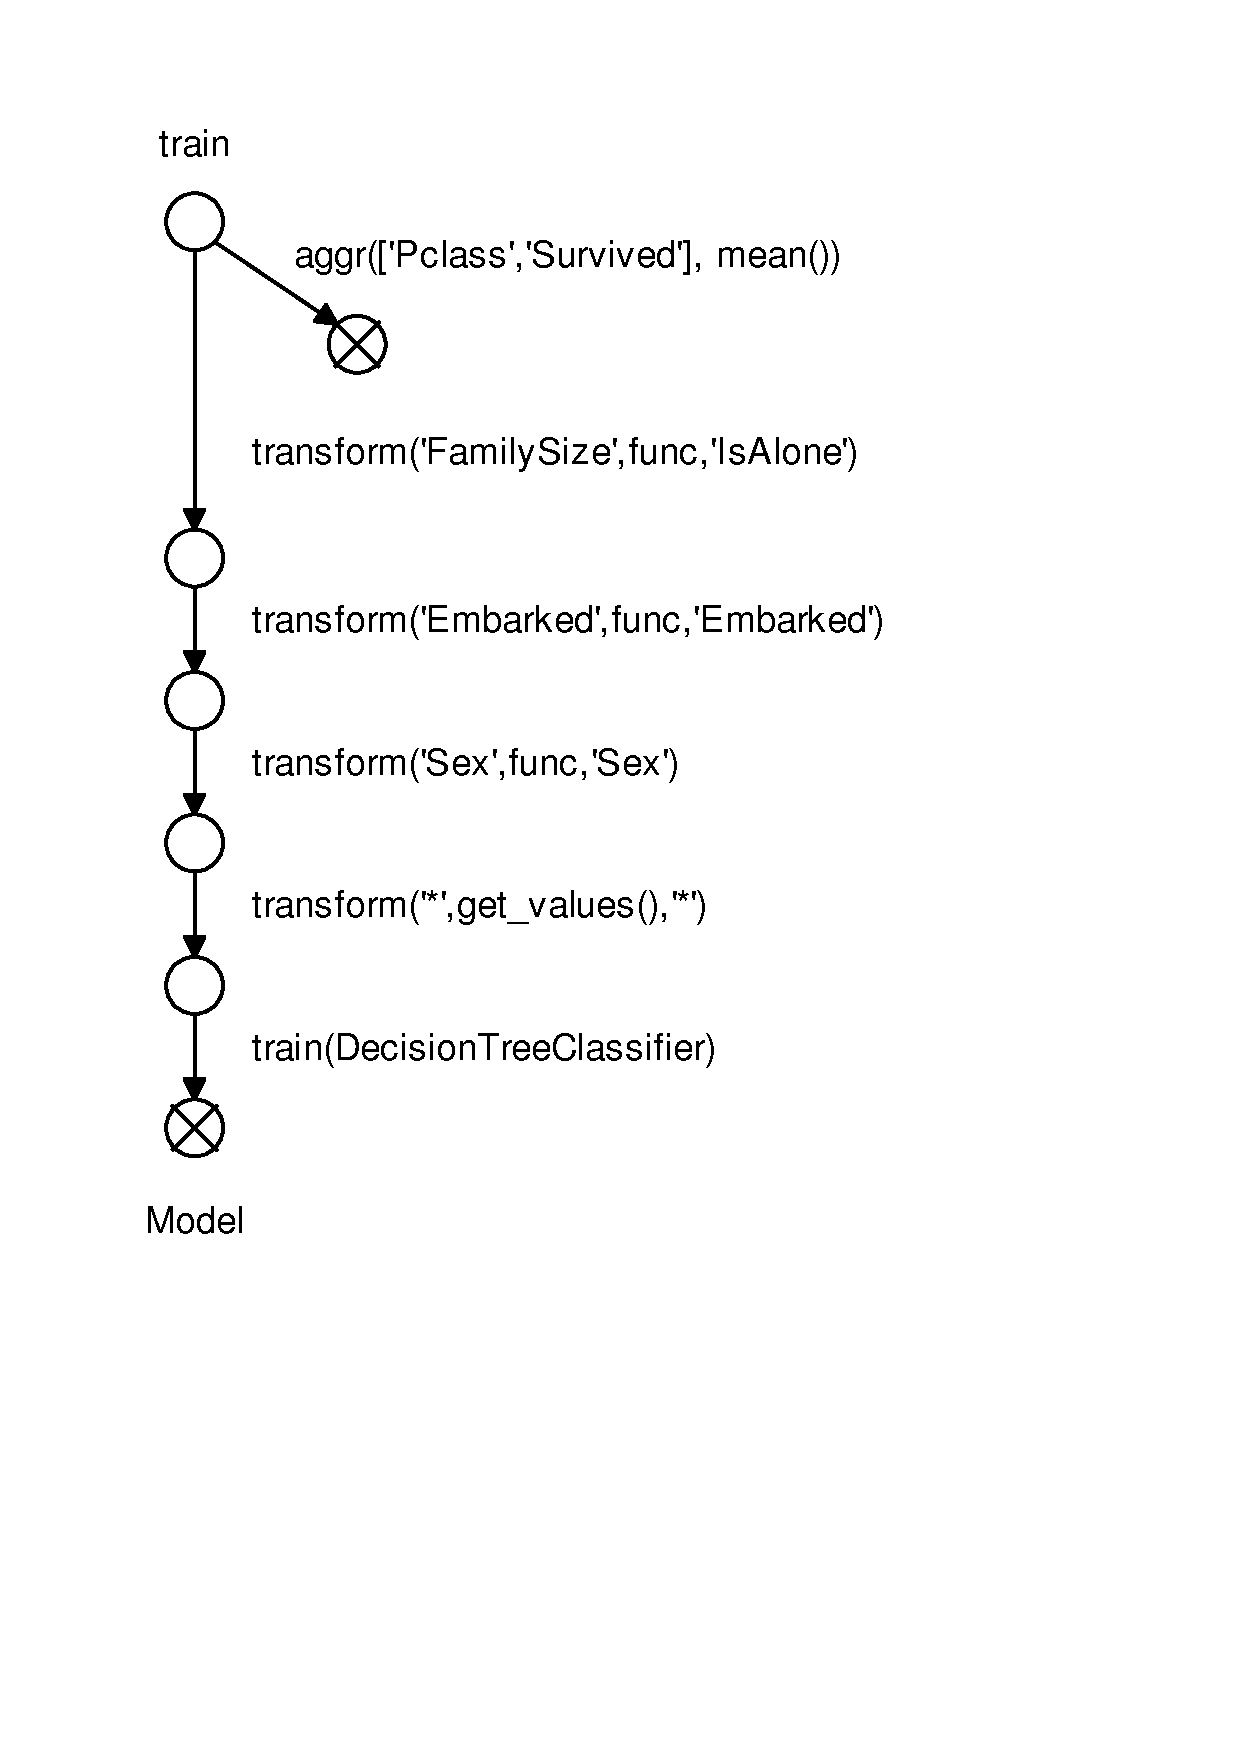
\includegraphics[width=0.6\columnwidth]{../images/experiment-graph}
\caption{Experiment graph constructed from the listing \ref{listing-experiment-graph}}
\label{fig-experiment-graph}
\end{figure}

\subsection{Materialization and Reuse of Operations}\label{sub-sec-materializaiton-of-operations}
Each operation on a data can be mapped to an edge $e$ (representing the operation) that connexts a vertex $v$ (representing the data) to another vertex $v'$ (representing the transformed data).
A series of operations on a data (a partial pipeline) can be translate to a path in the graph, starting from the vertex representing the data ($v$), along an ordered list of edges, each representing one operation ($e_i$), resulting in the final data ($v'$). 
Each edge in the path connects the source data ($v_i$) to a intermediate transformed data ($v_{i+1}$).
Using this representation, we can search the graph constructed from the experiment database to look for reuse opportunities.

Algorithm \ref{alg-reuse} shows the process of detecting reuse for one operations.
\begin{algorithm}
\caption{Reuse algorithm}\label{alg-reuse}
\begin{algorithmic}[1]
\Require vertex $d$ representing the dataset, edge $e$ representing the operation, graph $G$ constructed from the experiment database
\Ensure vertex $d'$ representing the transformed data (returns the input vertex if reuse is not possible)
\Function{Reuse}{$d,e,G$}
	\If {$d \in G$}
		\For {$i$ in $out\_edges(G,d)$}
			 	\If {$i = e$}
			 		 \State \textbf{return} $i.destination$
			 	\EndIf
		\EndFor
	\EndIf
   \State \textbf{return} $d$
\EndFunction
\end{algorithmic}
\end{algorithm}

 
\begin{algorithm}
\caption{Path Reuse algorithm}\label{alg-reuse-partial_pipeline}
\begin{algorithmic}[1]
\Require vertex $d$ representing the dataset, edge list $E$ representing the sorted list of operations, graph $G$ constructed from the experiment database
\Ensure vertex $d'$ representing the transformed data to use
\Function{Reuse\_path}{$d,E,G$}
	\State $next$ = $REUSE(d, E[0],G)$
	\If {$next = d$}
		\State \textbf{return} $next$
	\ElsIf {$E.size > 1$}
		\State \textbf{return} $REUSE\_PATH(next, E - E[0], G)$
	\Else
		\State \textbf{return} $next$
	\EndIf
\EndFunction
\end{algorithmic}
\end{algorithm}

Algorithm \ref{alg-reuse-partial_pipeline} shows the process of detecting reuse opportunities given a path.

\subsection{The Problem of Unaligned Pipelines}
The reuse algorithm presented in Section \ref{sub-sec-materializaiton-of-operations} has one drawback that affects real-world use cases.
In our analysis of the Kaggle scripts, we realize that although a large portions of the operations are the same across multiple notebooks, sometimes there are slight differences.
Users tend to apply the operations in arbitrary order and while the final results may be the same the process of arriving at the result is different.
There are two common problematic scenarios that occur while users are writing scripts.
Throughout our analysis, we further realize that many of the operations are applied to columns and re-order some of the operations does not affect the final result.
Figure \ref{fig-unaligned-operations} shows the two scenarios that may happen.
Although in both scenarios the operations can be reused, the algorithm is not able to detect them as the data nodes involved in the operations are different. 
Current graph consists of the original training dataset, and 4 operations, where oper\_1, oper\_2, and oper\_3 transform different columns.
In scenario 1, a new user perform two transformations that also operate on different columns and then transforms the resulting data using oper\_1, oper\_2, and oper\_3.
In scenario 2, the same transformations (oper\_1, oper\_2, and oper\_3) are applied to the training data.
However, the order of the transformations are different.
Simple reuse algorithms (Algorithms \ref{alg-reuse}, \ref{alg-reuse-partial_pipeline}) are not able to detect the reuse opportunities in these two scenarios.

\begin{figure}
\centering
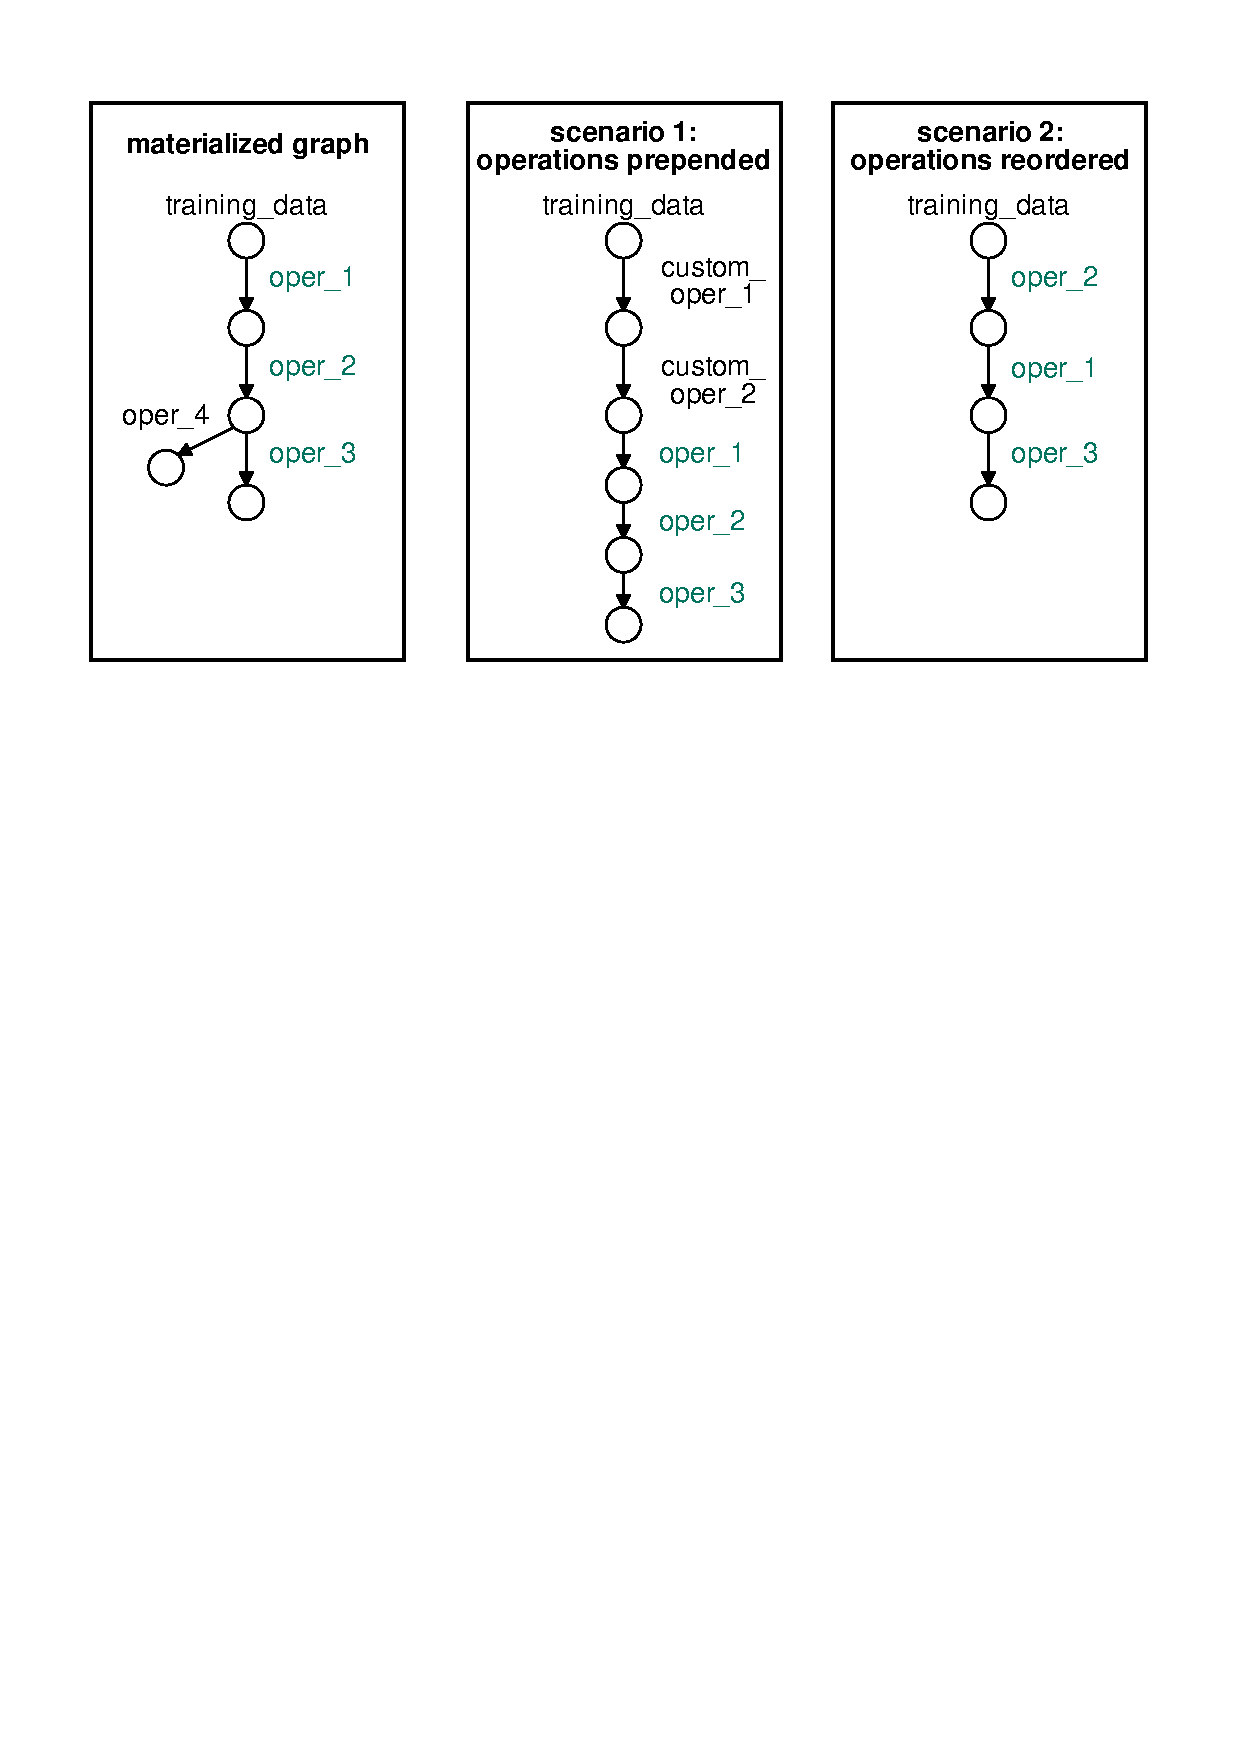
\includegraphics[width=\columnwidth]{../images/unaligned-operations}
\caption{Two scenarios that direct reuse cannot be applied}
\label{fig-unaligned-operations}
\end{figure}

To apply reuse in these scenarios we have augment the experiment graph to capture such mutual-exclusive transformations.

\subsection{Augmented Experiment Graph}
In this section, we explain our approach for extending the graph $G$, constructed from the experiment database, to capture the operations that are order-independent and therefore, enabling our reuse algorithms to be able in these scenarios as well.
In our approach, we augment the graph $G$, with edges that connect nodes that can be derived from earlier nodes using the same transformation.
Algorithms \ref{alg-add-augment-graph} and \ref{alg-augment-graph} show the procedure for adding a new transformation and augmenting the graph.
When a new transformation is added, the graph is traversed in the opposite direction of the edges starting from the current data node (source of the transformation).
If the immediate preceding nodes contain all the columns involved in the transformation (i.e. \textit{active\_columns}), an edge is added to the graph.
The process continues until a vertex does not contain all the active columns, or the traversal reaches the root node (i.e., $in\_edges(G,d) = \emptyset$).

\begin{algorithm}
\caption{Add and Augment Graph algorithm}\label{alg-add-augment-graph}
\begin{algorithmic}[1]
\Require vertex $d$ representing the dataset, edge $e$ representing the operation, graph $G$ constructed from the experiment database
\Ensure Graph $G$ containing the new transformation and all the augment edges
\Function{Add\_And\_Augment\_Graph}{$d,e,G$}
	\State $G = G \cup e$ \Comment{Add the transformation to the graph}
	\State $destination = e.destination$ 
	\State $tf=e.transformation\_function$ 
	\State $ac=e.active\_columns$ \Comment{columns involved in e}
	\State \textbf{return} $AUGMENT\_GRAPH(d, destination,ac, tf, G)$   \Comment{Call the recursive augment procedure}
\EndFunction
\end{algorithmic}
\end{algorithm}

\begin{algorithm}
\caption{Augment Graph algorithm}\label{alg-augment-graph}
\begin{algorithmic}[1]
\Require vertex $d$ representing the dataset, vertex $d'$ representing the transformed dataset, active columns $ac$ representing the list of columns involved in the operation, transformation function $tf$, graph $G$ constructed from the experiment database
\Ensure Graph $G$ representing the augmented graph
\Function{Augment\_Graph}{$d,d',ac,tf,G$}
	\For {$n$ in $in\_edges(G,d)$ }
		\If {$n.columns = ac$}
			\State  $new\_edge=Edge(n.start, d', ac,tf)$
			\State $G = G \cup new_edge$
			\State  $AUGMENT\_GRAPH(n.start, d',ac, tf,G)$
		\EndIf
	\EndFor
   \State \textbf{return} $G$
\EndFunction
\end{algorithmic}
\end{algorithm}


%\subsection{Materialization of Grid Search}
%\todo[inline]{Incomplete}
%In order to analyze whether or not we should materialize parts of the grid search, we first have to unpack it, and compare it with other grid search.
%Then, similar to Section \ref{sub-sec-materialization-of-transformed-data}, we materialize the parts that are executed frequently.
%
%%\subsection{Guided Grid-Search}
%%\todo[inline]{just an idea}
%%By extracting correlation between different parameters and the model quality we can provided a guided grid search, where we can provide some estimate or show the effects of a hyperparameter range on the model quality